\documentclass[11pt]{article}
\usepackage[sort]{natbib}
\usepackage{bm,amsmath,bbm,amsfonts,nicefrac,latexsym,amsmath,amsfonts,amsbsy,amscd,amsxtra,amsgen,amsopn,bbm,amsthm,amssymb,graphicx, color, caption, subcaption}
\usepackage{fancyhdr, pbox}
\usepackage[margin=0.7in]{geometry}
\usepackage[english]{babel}
\usepackage[section]{placeins}
\usepackage{wrapfig}
\usepackage{lscape}
\usepackage{rotating}
\usepackage{epstopdf}
\bibliographystyle{plainnat}

\title{New Figure Ideas}
\author{Ewan Pinnington}

\newtheorem{theorem}{Theorem}[section]
\newtheorem*{defn}{Definition}


\begin{document}

\maketitle


\begin{figure}
    \centering
    \begin{subfigure}[b]{0.49\textwidth}
        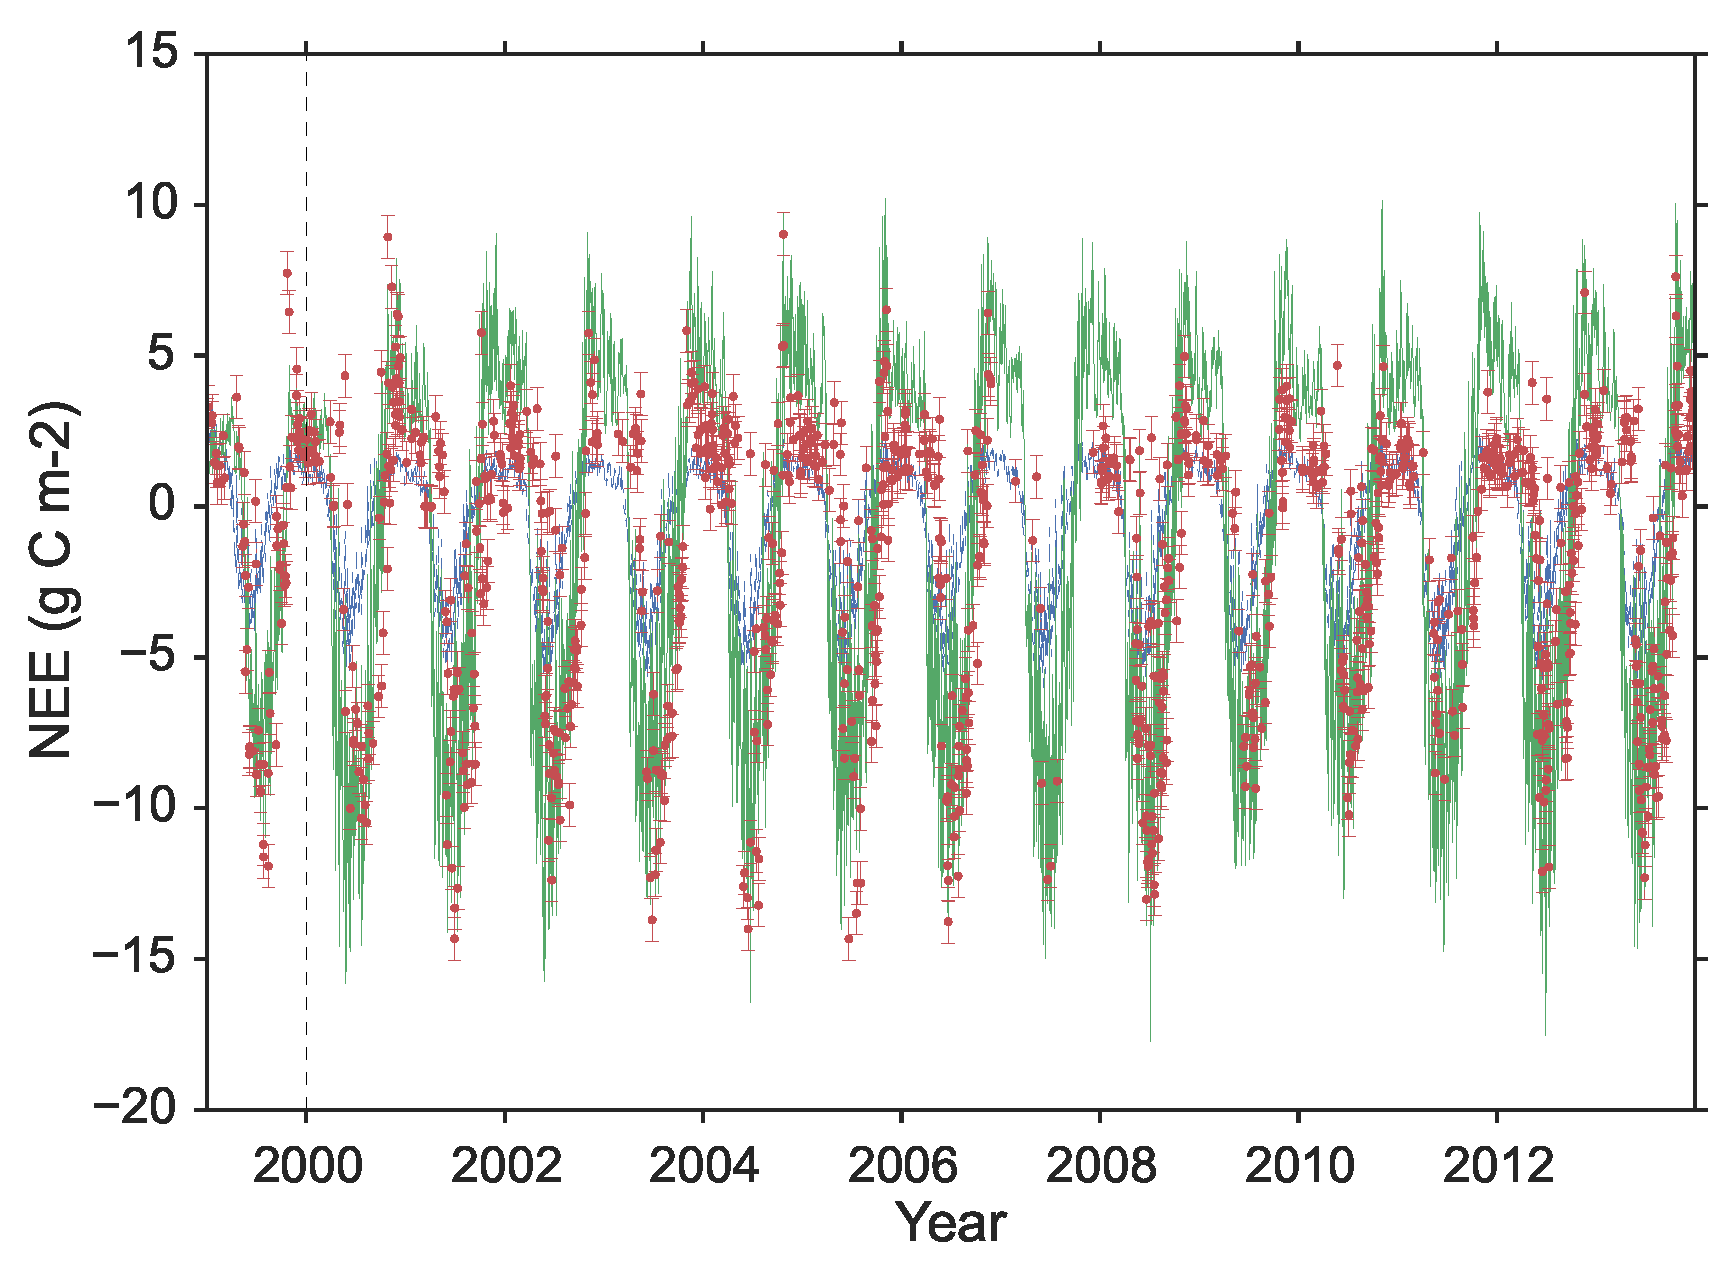
\includegraphics[width=\textwidth]{A4dvar.eps}
        \caption{Experiment A}
        \label{fig:4dvardiagBR}
    \end{subfigure}
    \begin{subfigure}[b]{0.49\textwidth}
        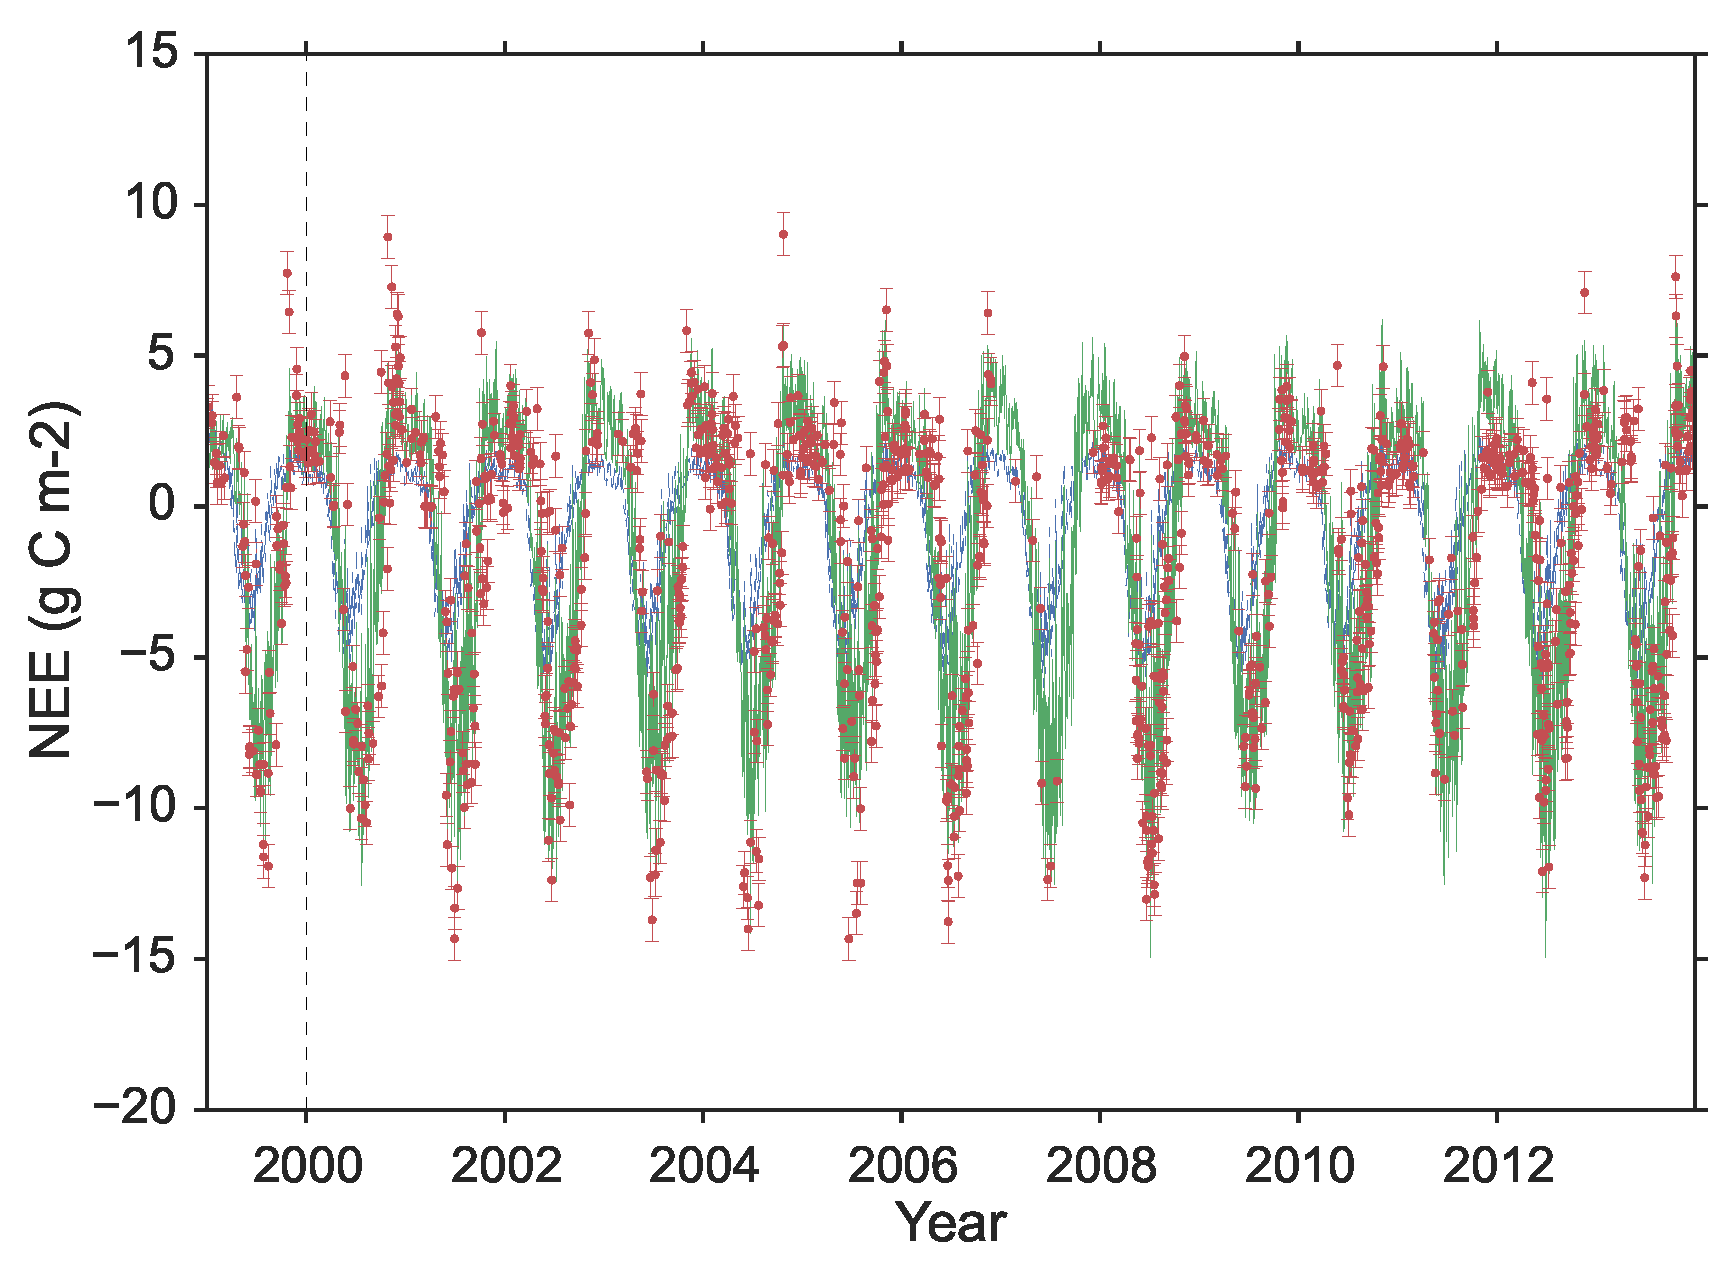
\includegraphics[width=\textwidth]{B4dvar.eps}
        \caption{Experiment B}
        \label{fig:4dvaredcBR}
    \end{subfigure}
    \begin{subfigure}[b]{0.49\textwidth}
        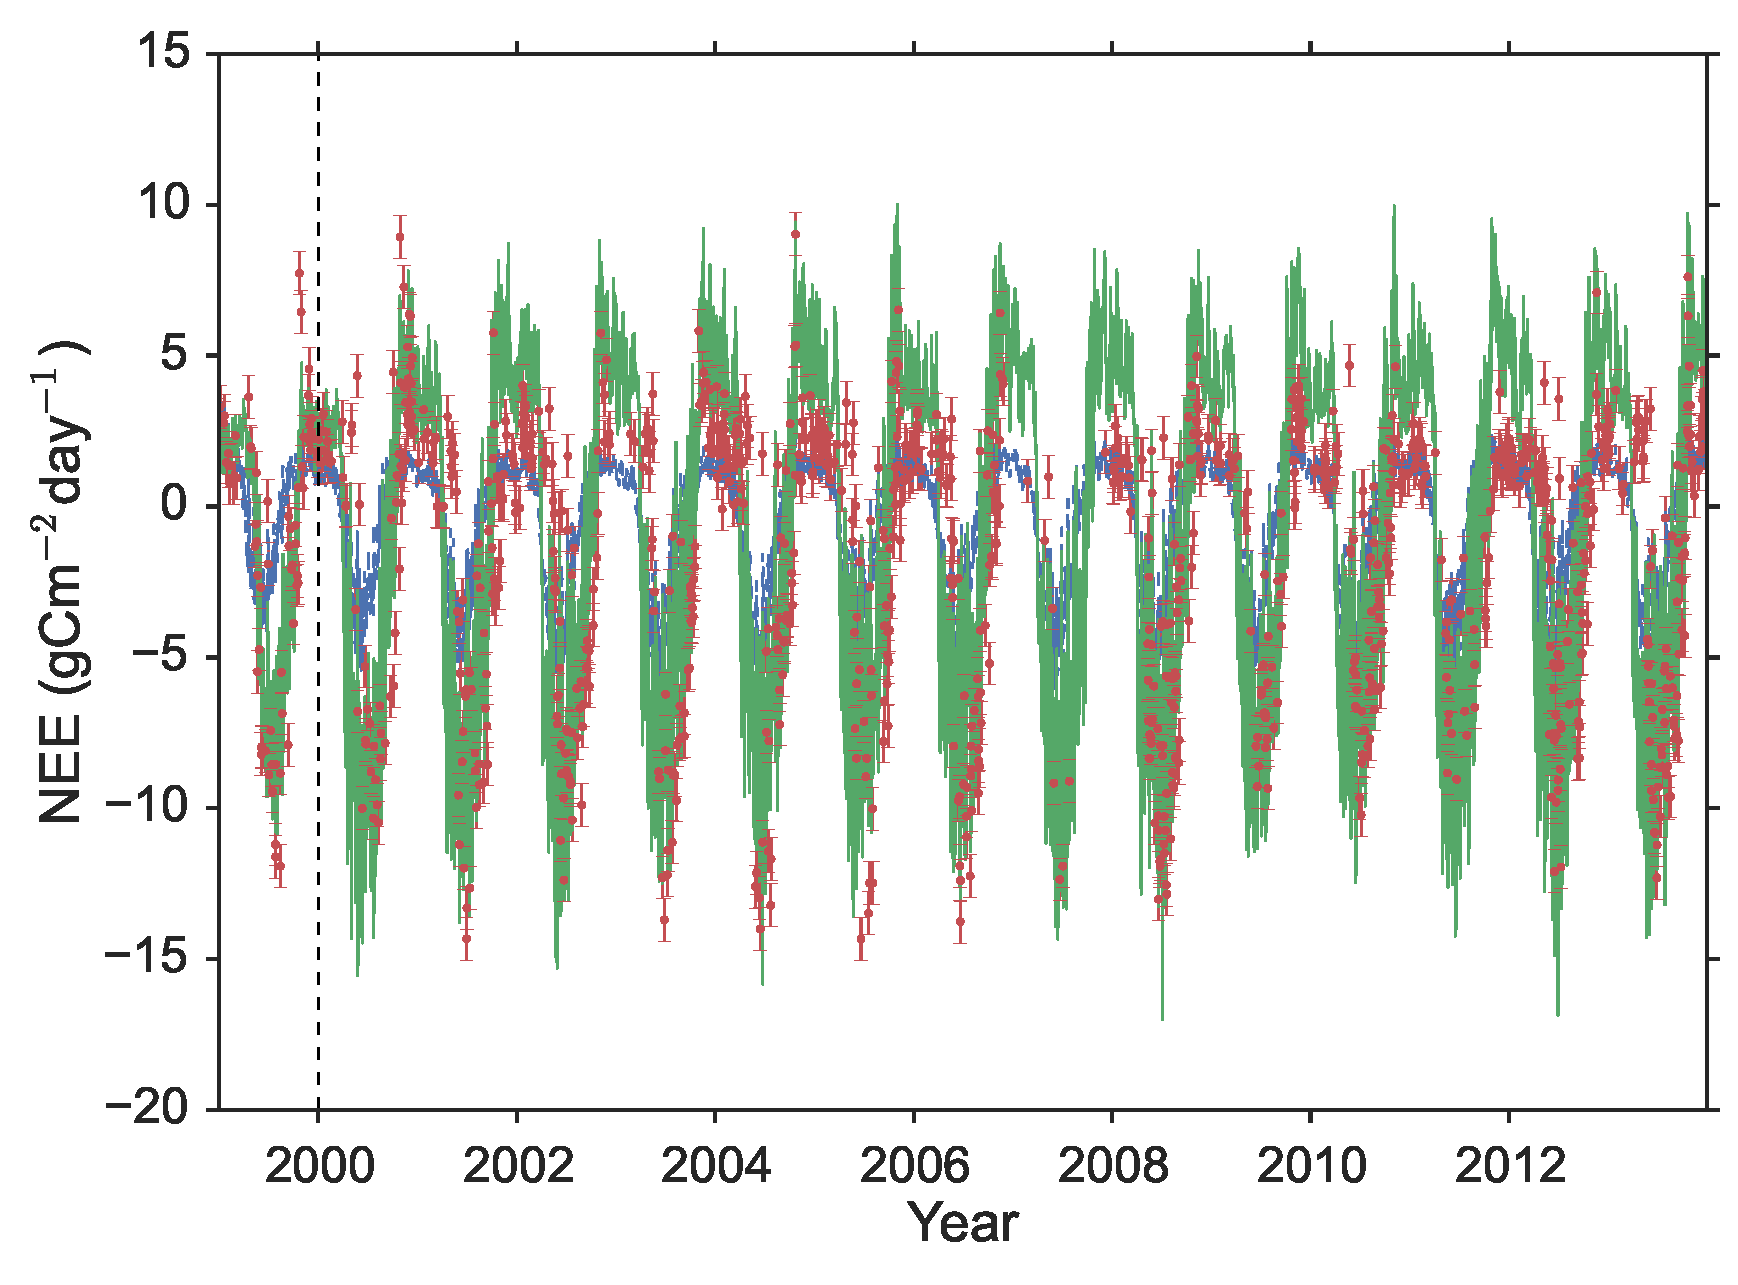
\includegraphics[width=\textwidth]{C4dvar.eps}
        \caption{Experiment C}
        \label{fig:4dvarBcorR}
    \end{subfigure}
    \begin{subfigure}[b]{0.49\textwidth}
        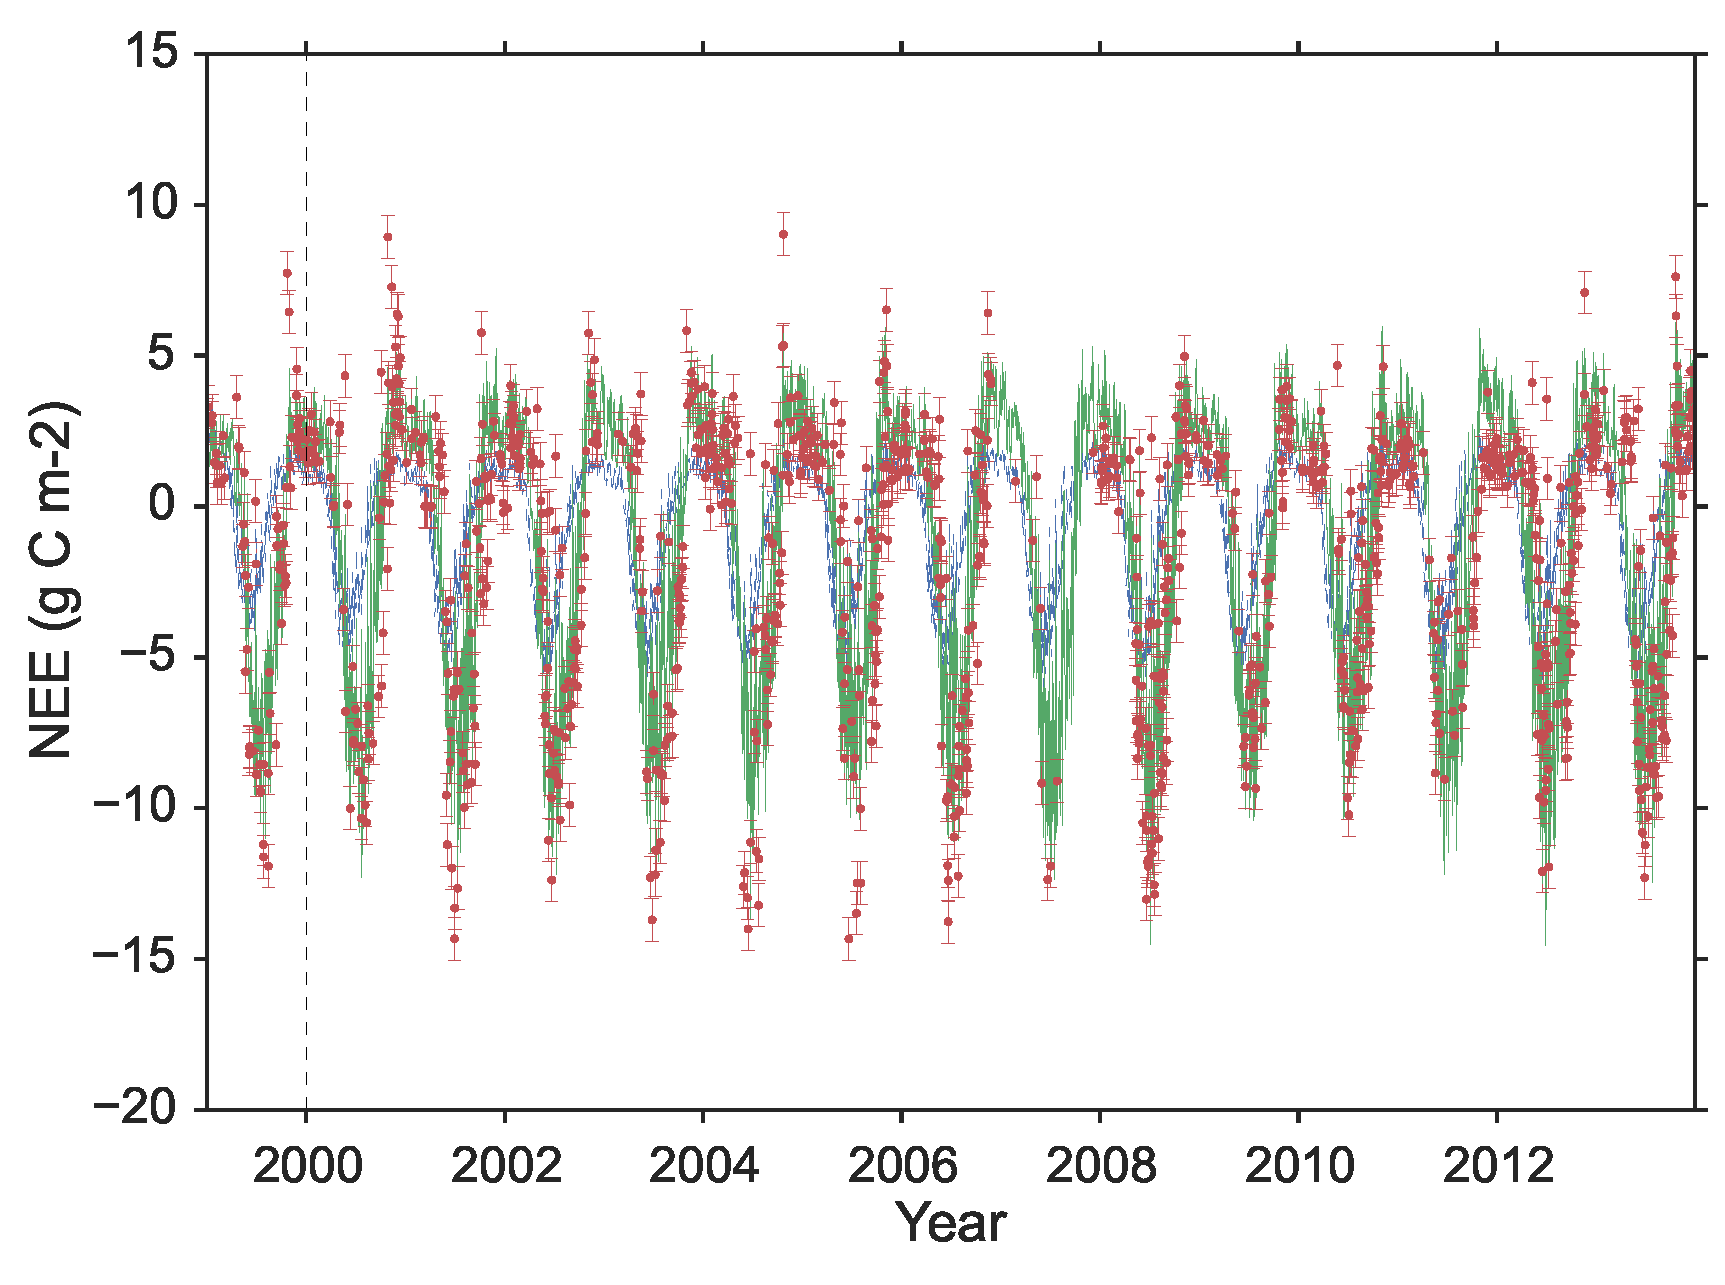
\includegraphics[width=\textwidth]{D4dvar.eps}
        \caption{Experiment D}
        \label{fig:4dvaredcBcorR}
    \end{subfigure}
    \caption{One year assimilation and fourteen year forecast of Alice Holt NEE with DALEC2, blue dotted line: background model trajectory, green line: analysis and forecast after assimilation, red dots: observations from Alice Holt flux site with error bars.}\label{fig:4dvar}
\end{figure}

\begin{figure}
    \centering
    \begin{subfigure}[b]{0.49\textwidth}
        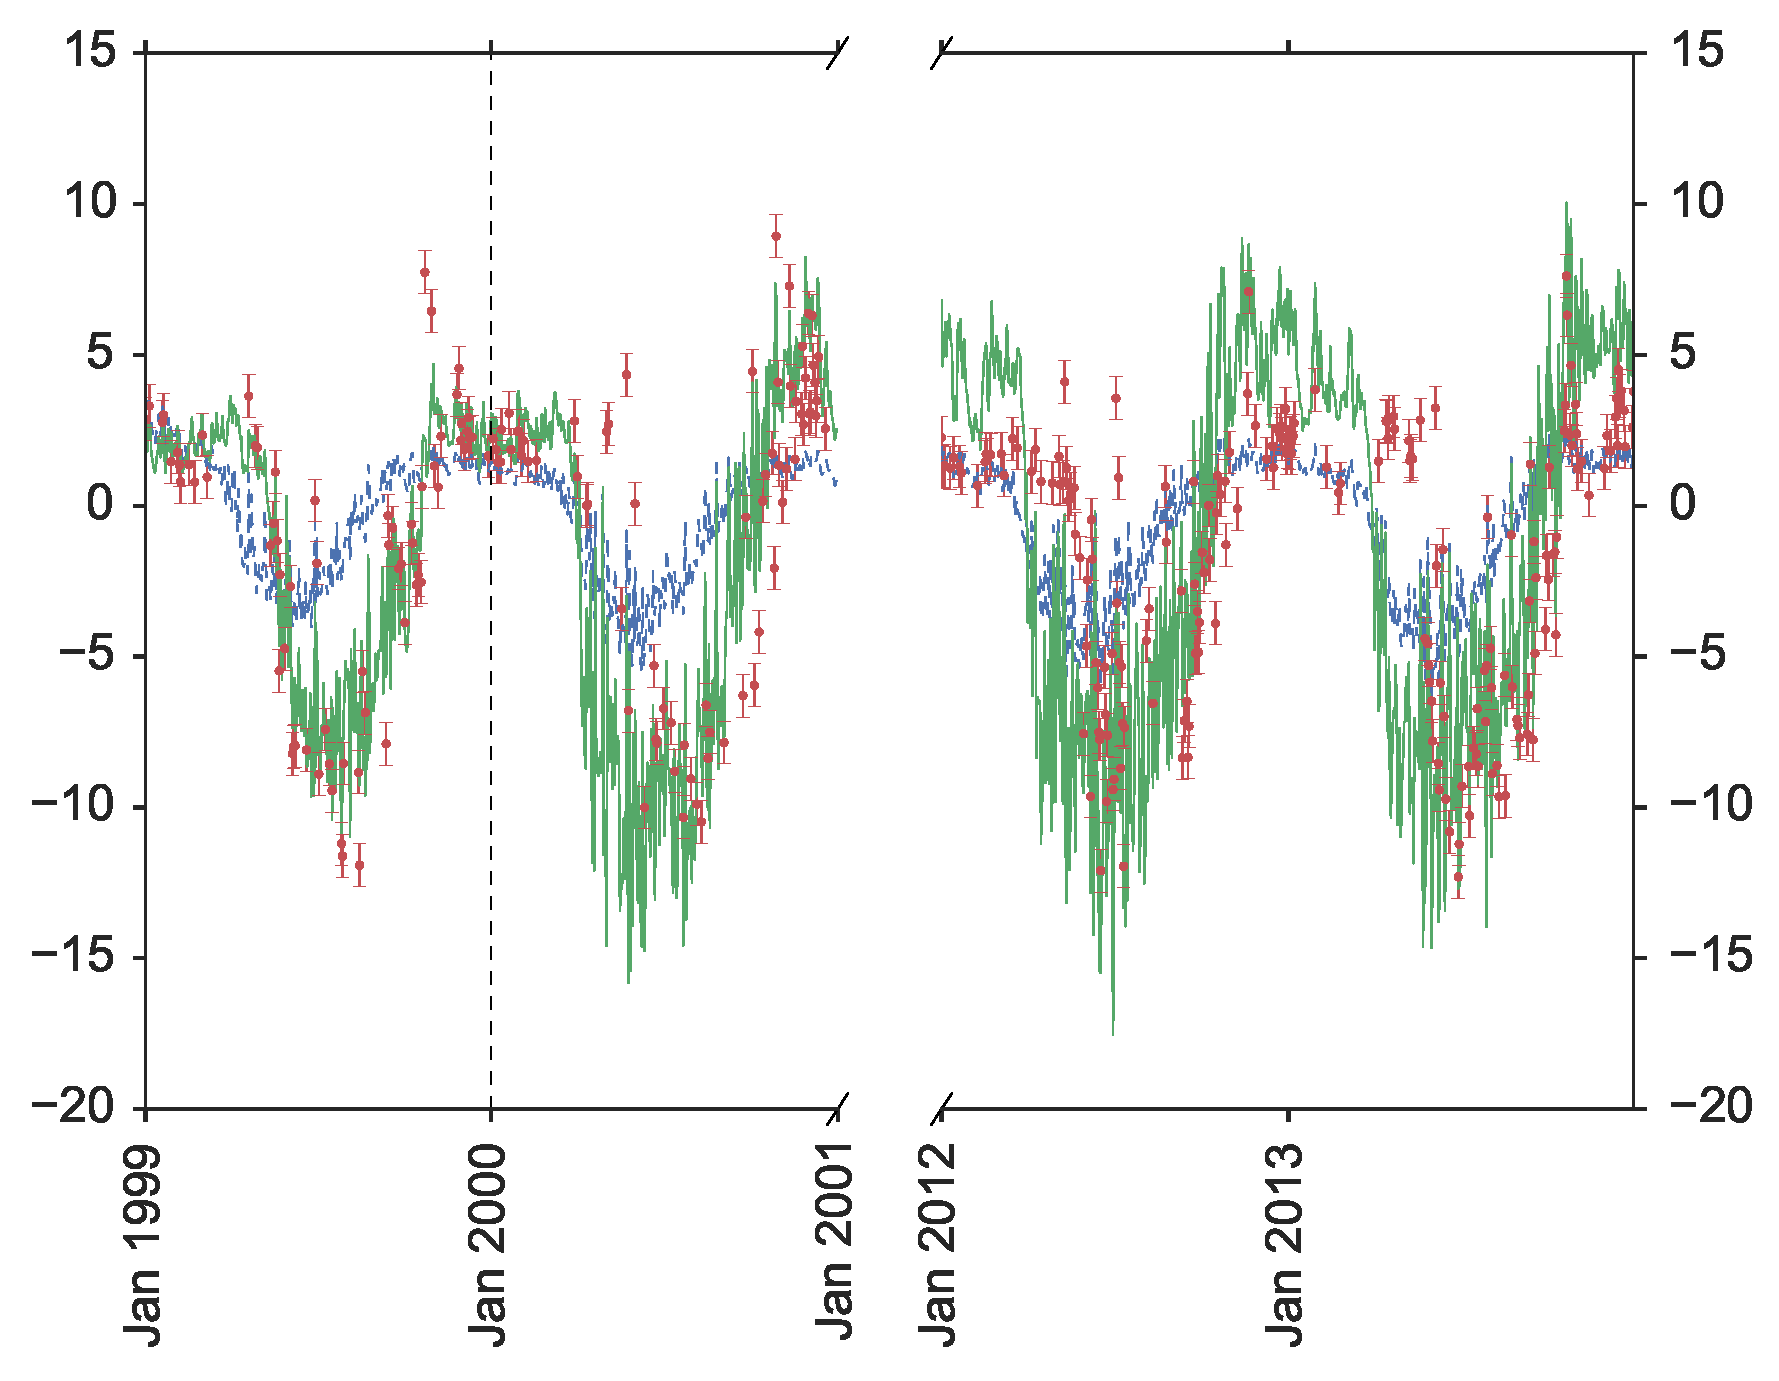
\includegraphics[width=\textwidth]{Abroke4dvar.eps}
        \caption{Experiment A}
        \label{fig:4dvardiagBR}
    \end{subfigure}
    \begin{subfigure}[b]{0.49\textwidth}
        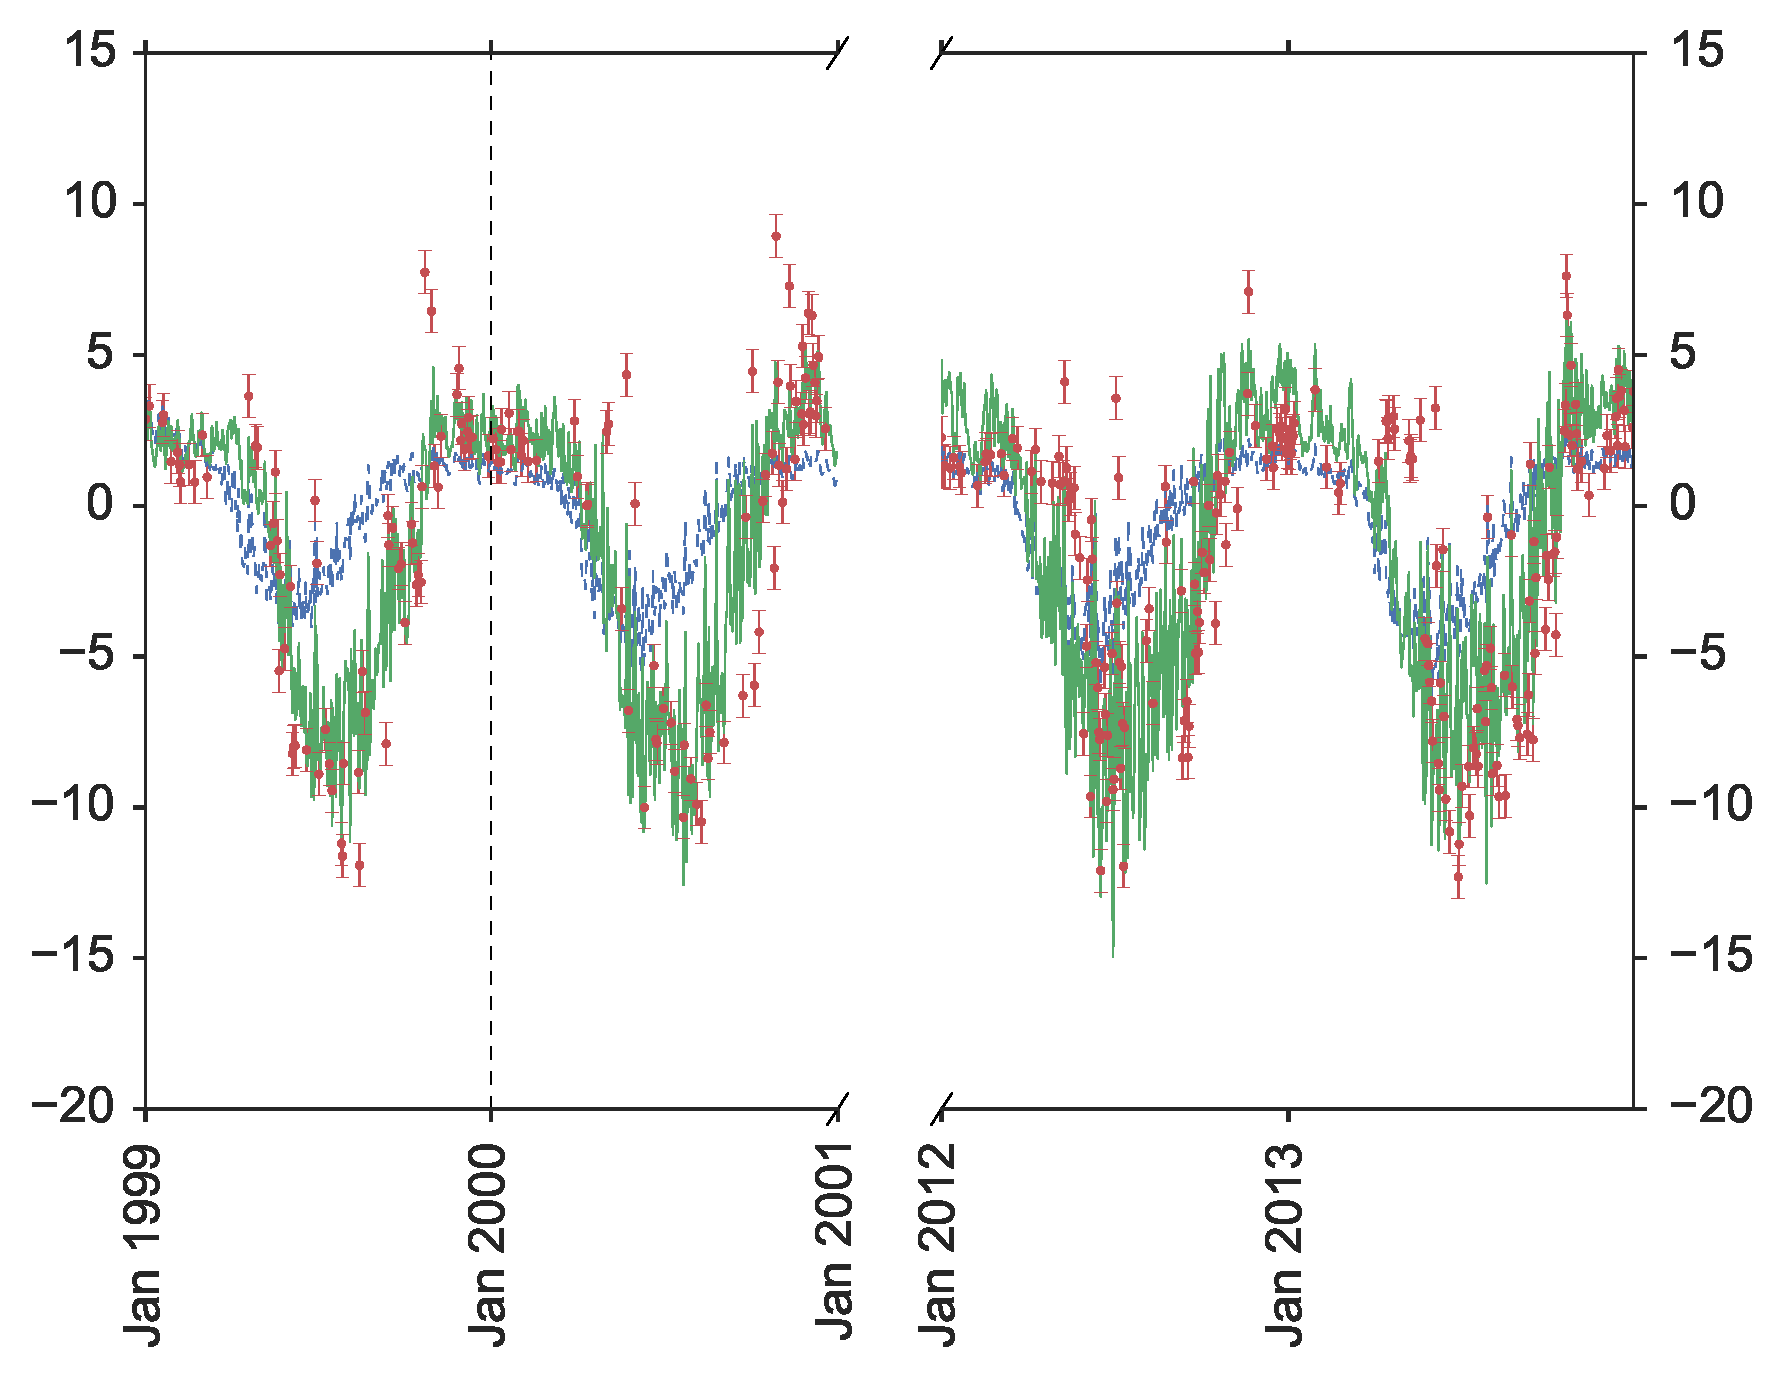
\includegraphics[width=\textwidth]{Bbroke4dvar.eps}
        \caption{Experiment B}
        \label{fig:4dvaredcBR}
    \end{subfigure}
    \begin{subfigure}[b]{0.49\textwidth}
        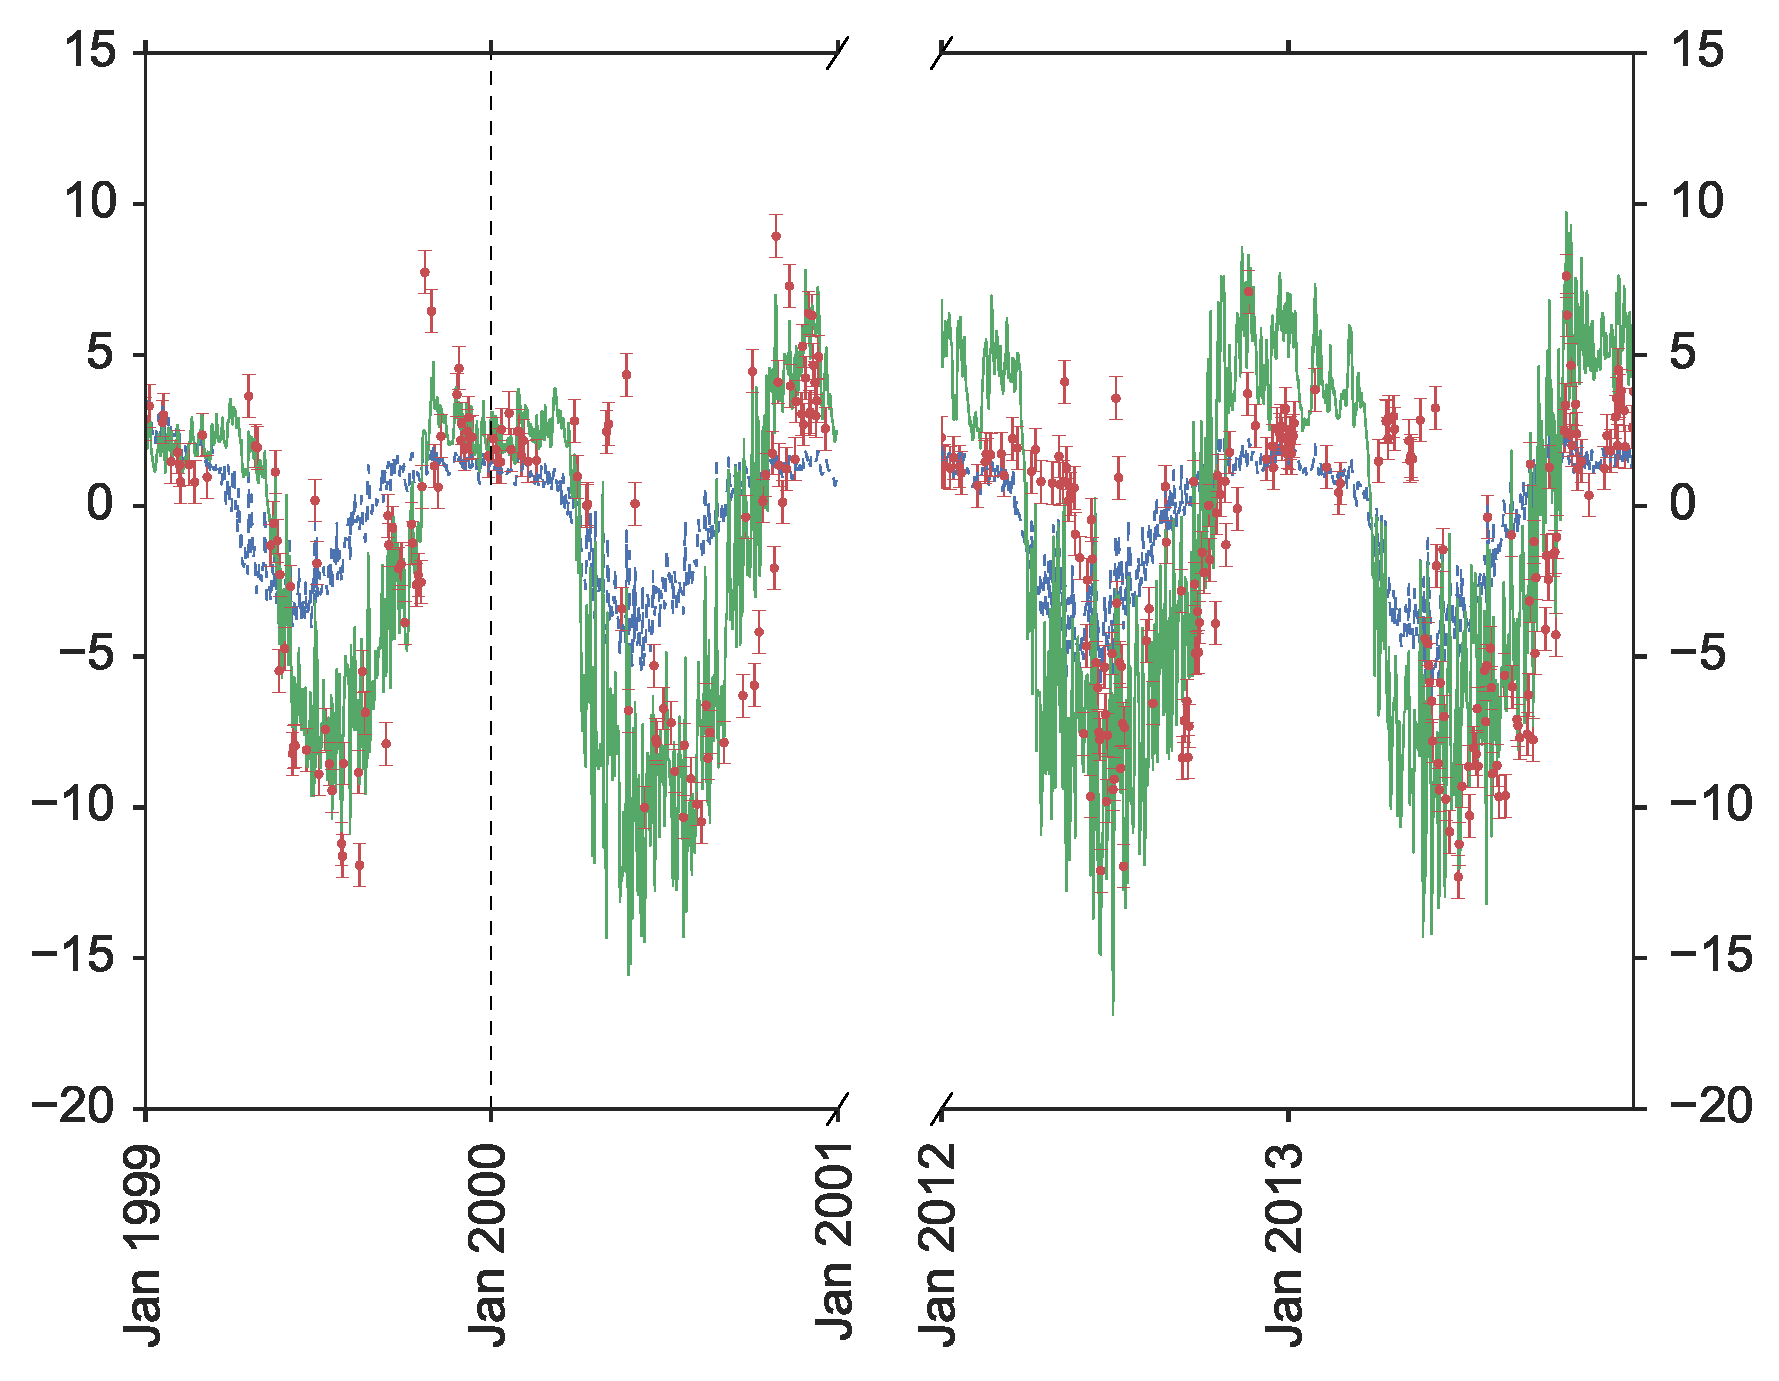
\includegraphics[width=\textwidth]{Cbroke4dvar.eps}
        \caption{Experiment C}
        \label{fig:4dvarBcorR}
    \end{subfigure}
    \begin{subfigure}[b]{0.49\textwidth}
        \includegraphics[width=\textwidth]{Dbroke4dvar.eps}
        \caption{Experiment D}
        \label{fig:4dvaredcBcorR}
    \end{subfigure}
    \caption{Broken: One year assimilation and fourteen year forecast of Alice Holt NEE with DALEC2, blue dotted line: background model trajectory, green line: analysis and forecast after assimilation, red dots: observations from Alice Holt flux site with error bars.}\label{fig:4dvar}
\end{figure}

\begin{figure}
    \centering
    \begin{subfigure}[b]{0.49\textwidth}
        \includegraphics[width=\textwidth]{Afscat.eps}
        \caption{Experiment A}
        \label{fig:forecastscatBR}
    \end{subfigure}
    \begin{subfigure}[b]{0.49\textwidth}
        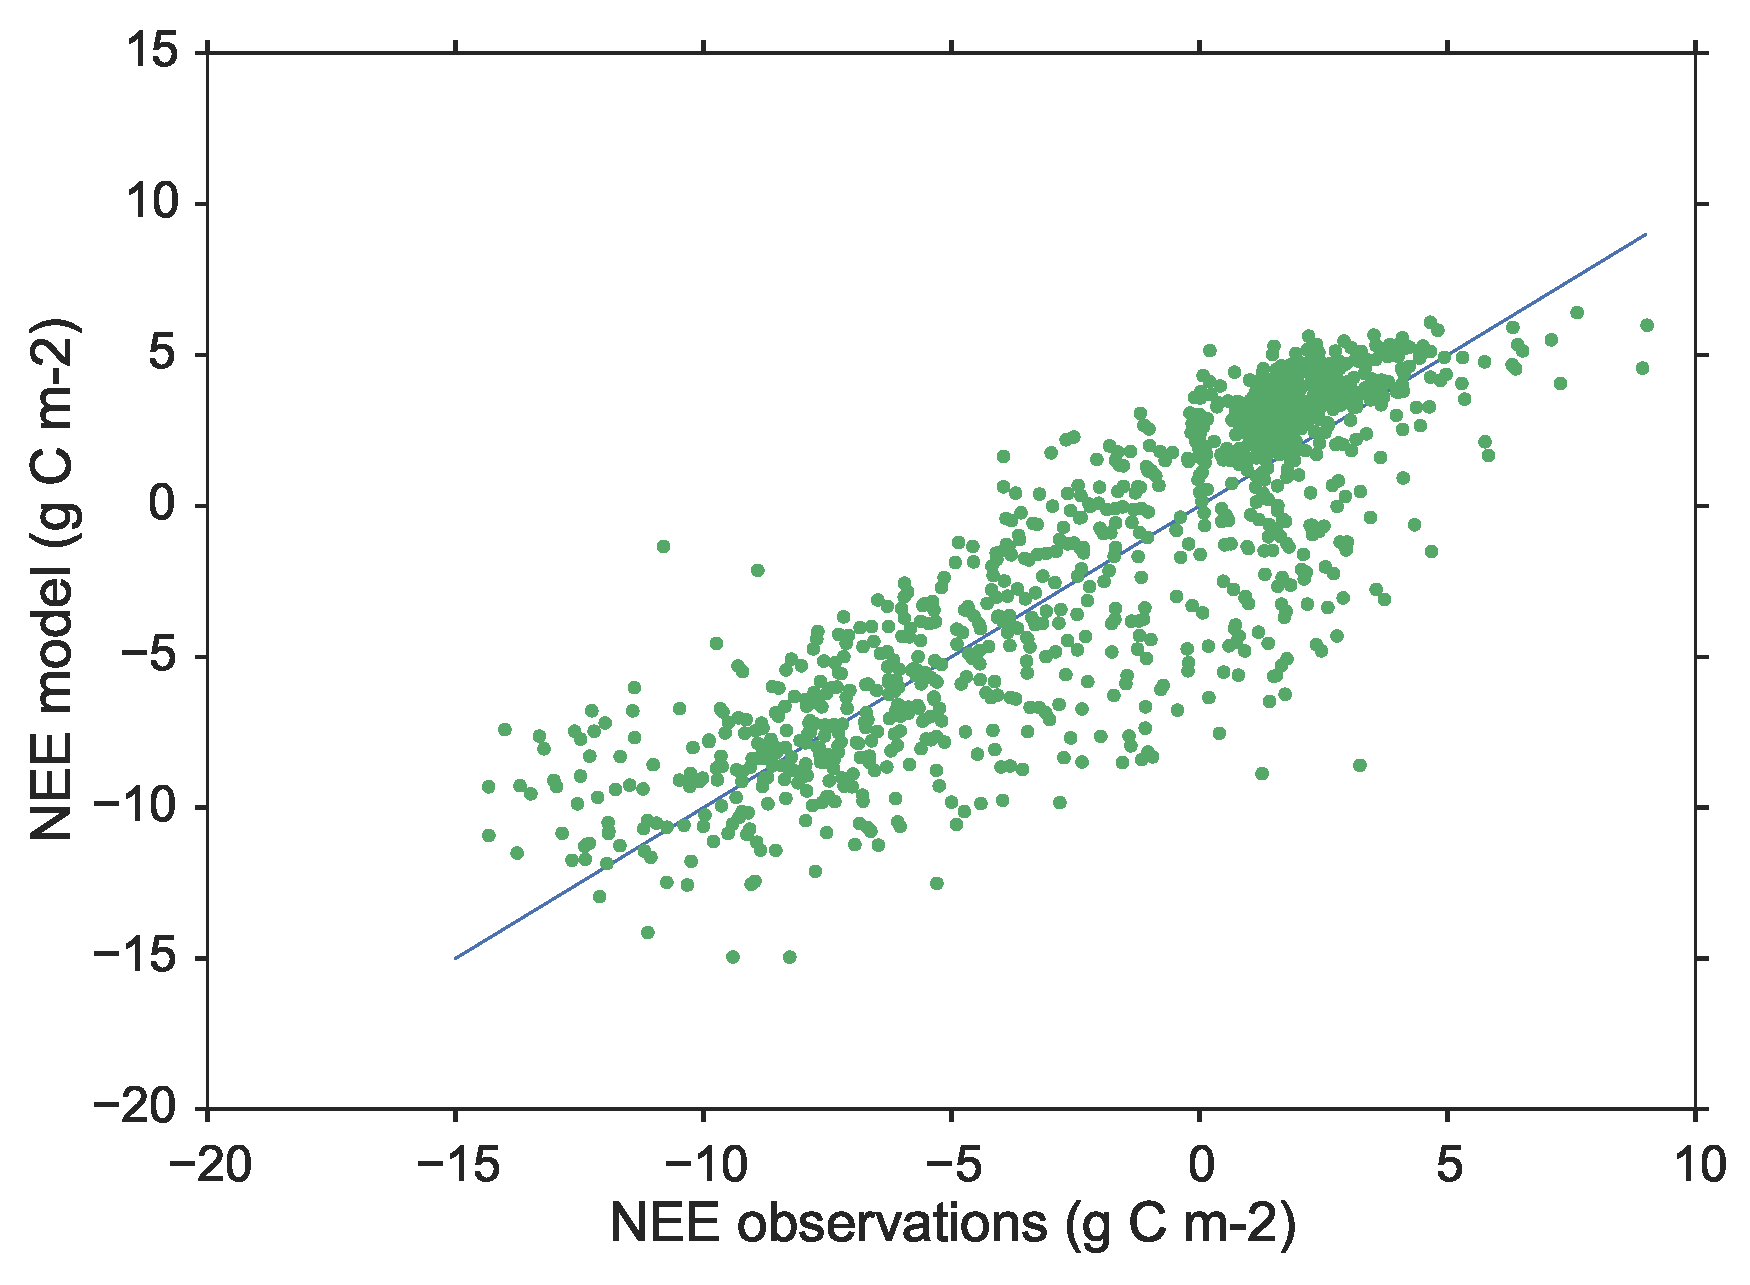
\includegraphics[width=\textwidth]{Bfscat.eps}
        \caption{Experiment B}
        \label{fig:forecastscatedcBR}
    \end{subfigure}
    \begin{subfigure}[b]{0.49\textwidth}
        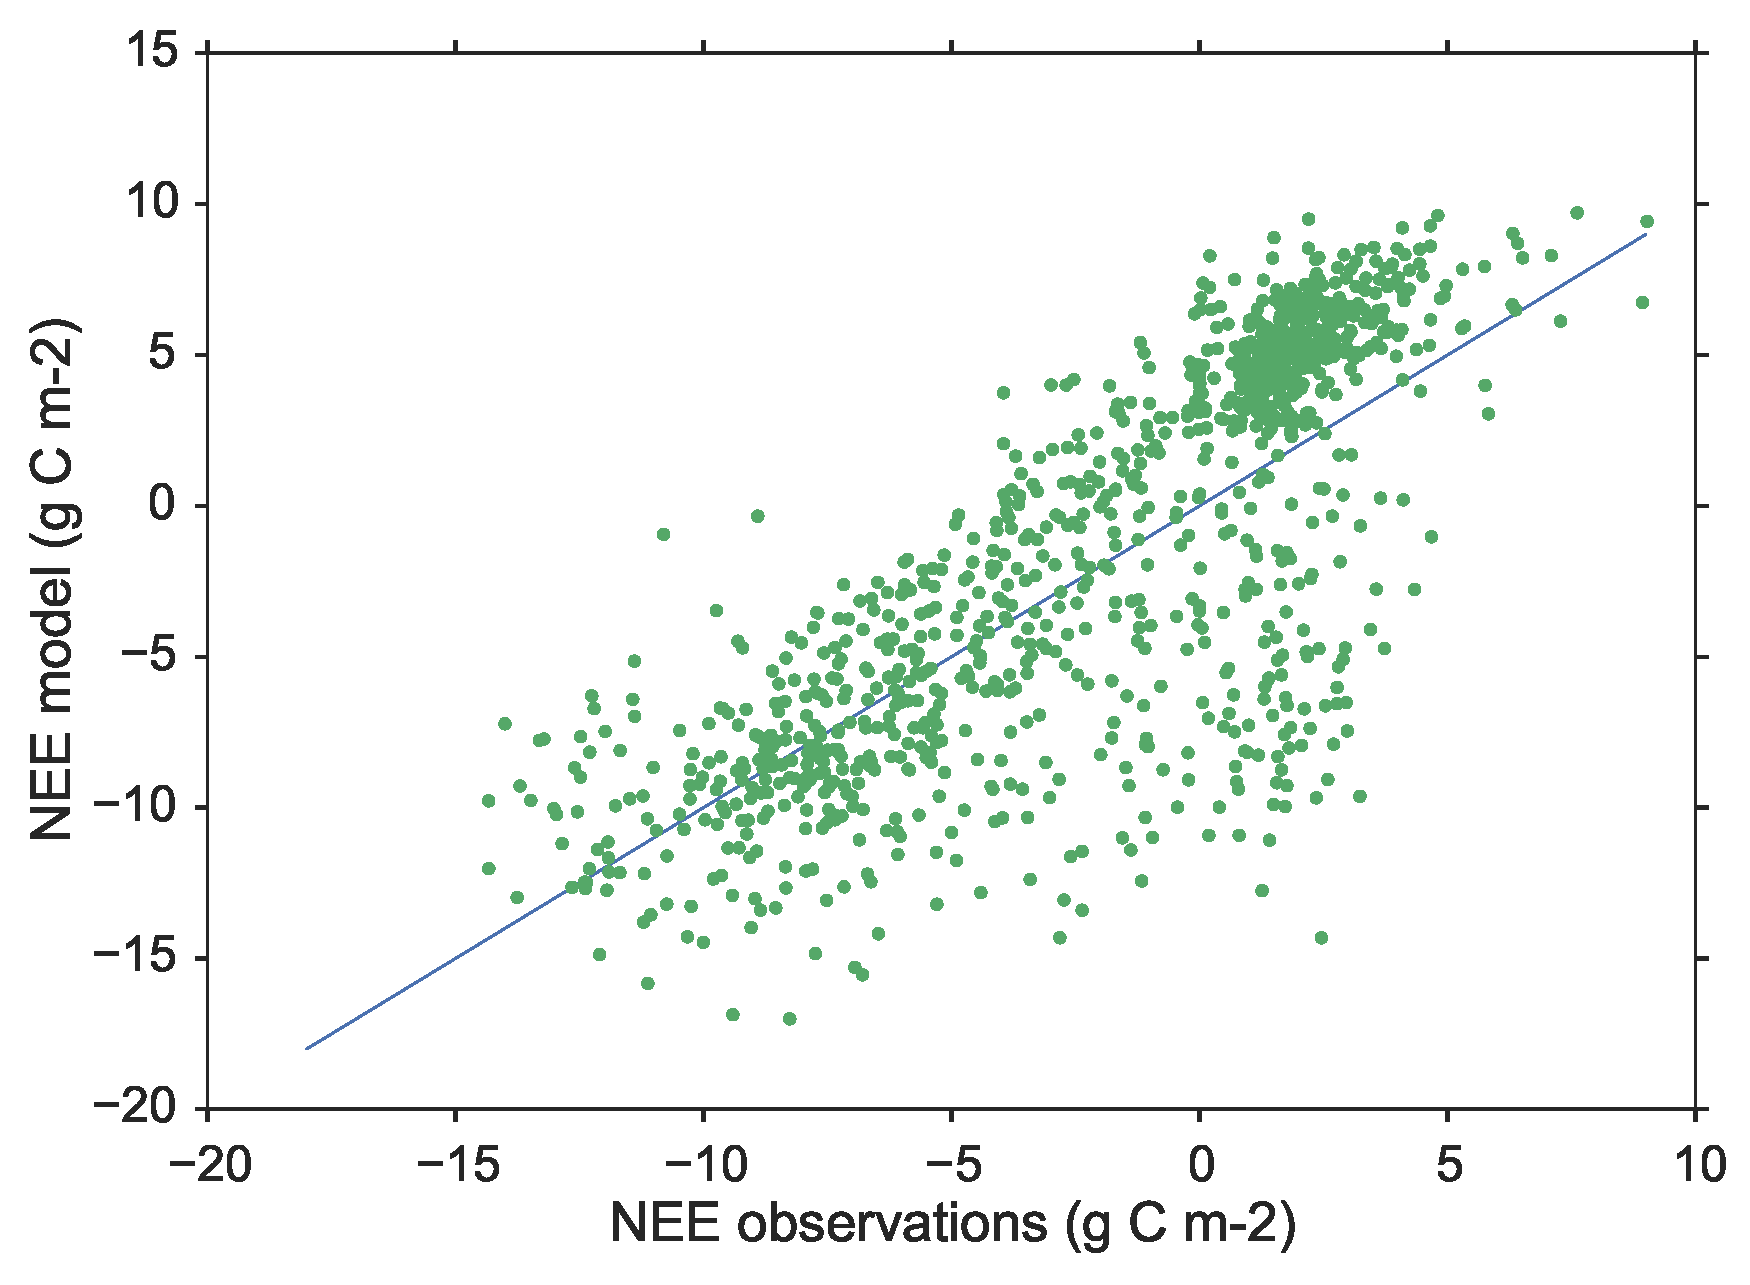
\includegraphics[width=\textwidth]{Cfscat.eps}
        \caption{Experiment C}
        \label{fig:forecastscatBcorR}
    \end{subfigure}
    \begin{subfigure}[b]{0.49\textwidth}
        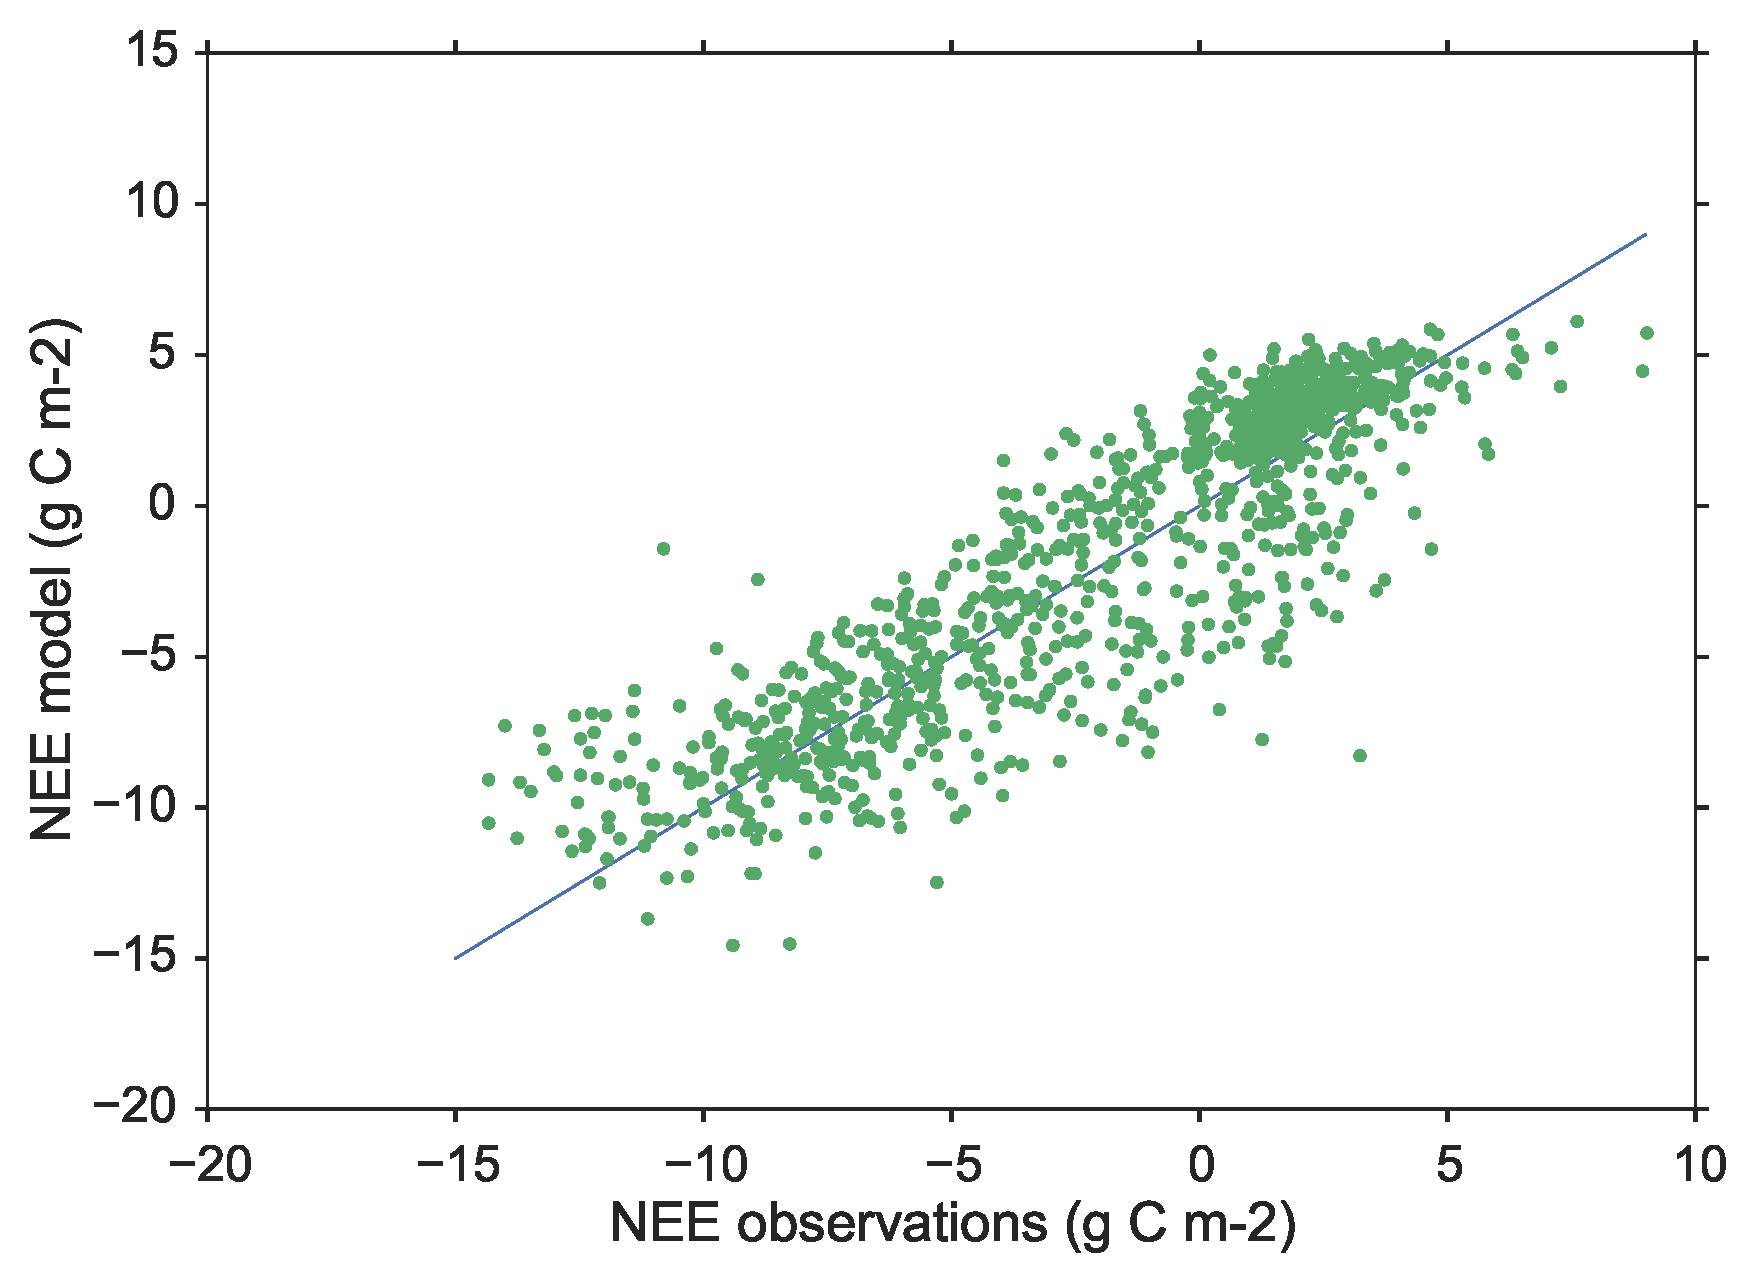
\includegraphics[width=\textwidth]{Dfscat.eps}
        \caption{Experiment D}
        \label{fig:forecastscatedcBcorR}
    \end{subfigure}
    \caption{Forecast scatter plot of modelled NEE vs. observations for 2000-2014 (green dots). Blue line represents the 1-1 line.}\label{fig:animals}
\end{figure}


\begin{table}[ht] 
\begin{center}
	\begin{tabular}{| l | l | l | l | l |}
	\hline
	Experiment & RMSE $( \text{gCm}^{-2})$ & Bias $( \text{gCm}^{-2})$ & Correlation coefficient & \pbox{5cm}{Minimisation function \\ evaluations} \\ \hline
	Background & $3.86$ & $-1.60$ & $0.70$ & $n/a$ \\ \hline
	A & $1.36$ & $-0.03$ & $0.96$ & $571$ \\ \hline
	B & $1.42$ & $-0.04$ & $0.95$ & $353$  \\ \hline
	C & $1.37$ & $-0.09$ & $0.96$ & $444$ \\ \hline
	D & $1.43$ & $-0.09$ & $0.95$ & $316$ \\ 
	\hline
	\end{tabular}
	\caption{Analysis (1999-2000) results for experiments and background when judged against observed NEE.}
	\label{table:exps_tab}
\end{center} 
\end{table}

\begin{table}[ht] 
\begin{center}
	\begin{tabular}{| l | l | l | l | l |}
	\hline
	Experiment & RMSE $( \text{gCm}^{-2})$ & Bias $( \text{gCm}^{-2})$ &  Correlation coefficient & \pbox{6cm}{Minimisation function \\ evaluations} \\ \hline
	Background & $3.86$ & $-1.36$ & $0.66$ & $n/a$ \\ \hline
	A & $4.22$ & $-0.30$ & $0.79$ & $571$ \\ \hline
	B & $2.56$ & $-0.20$ & $0.87$ & $353$  \\ \hline
	C & $4.09$ & $-0.51$ & $0.78$ & $444$ \\ \hline
	D & $2.38$ & $-0.33$ & $0.88$ & $316$ \\ 
	\hline
	\end{tabular}
	\caption{Forecast (2000-2014) results for experiments and background when judged against observed NEE.}
	\label{table:exps_tab}
\end{center} 
\end{table}

\begin{figure}[ht]
    \centering
    \includegraphics[width=0.8\textwidth]{inc.eps}
    \caption{Analysis increment for the four experiments.}
    \label{fig:testgradcostone}
\end{figure}

\section*{Appendix}

\begin{table}[ht] 
\begin{center}
	\begin{tabular}{| l | l | l | l | l | l |}
	\hline
	Parameter & Background & A & B & C &  D \\ \hline
$\theta_{min}$ & $9.810e-04$ & $1.000e-05$ & $1.000e-05$ & $1.000e-05$ & $1.000e-05$ \\ \hline
$f_{auto}$ & $5.190e-01$ & $3.000e-01$ & $3.089e-01$ & $3.000e-01$ & $3.134e-01$ \\ \hline
$f_{fol}$ & $1.086e-01$ & $1.640e-01$ & $3.025e-01$ & $1.822e-01$ & $3.006e-01$ \\ \hline
$f_{roo}$ & $4.844e-01$ & $3.886e-01$ & $4.398e-01$ & $4.298e-01$ & $4.452e-01$ \\ \hline
$c_{lspan}$ & $1.200e+00$ & $1.000e+00$ & $1.026e+00$ & $1.000e+00$ & $1.023e+00$ \\ \hline
$\theta_{woo}$ & $1.013e-04$ & $1.185e-04$ & $1.228e-04$ & $1.254e-04$ & $1.228e-04$ \\ \hline
$\theta_{roo}$ & $3.225e-03$ & $4.977e-03$ & $5.136e-03$ & $5.070e-03$ & $5.041e-03$ \\ \hline
$\theta_{lit}$ & $3.442e-03$ & $2.688e-03$ & $1.601e-03$ & $2.107e-03$ & $1.563e-03$ \\ \hline
$\theta_{som}$ & $1.113e-04$ & $1.873e-04$ & $1.443e-04$ & $1.914e-04$ & $1.482e-04$ \\ \hline
$\Theta$ & $4.147e-02$ & $8.000e-02$ & $7.697e-02$ & $8.000e-02$ & $7.616e-02$ \\ \hline
$c_{eff}$ & $7.144e+01$ & $1.000e+02$ & $9.347e+01$ & $1.000e+02$ & $9.276e+01$ \\ \hline
$d_{onset}$ & $1.158e+02$ & $1.196e+02$ & $1.237e+02$ & $1.194e+02$ & $1.230e+02$ \\ \hline
$f_{lab}$ & $3.204e-01$ & $3.801e-01$ & $1.000e-02$ & $3.707e-01$ & $1.000e-02$ \\ \hline
$c_{ronset}$ & $4.134e+01$ & $2.752e+01$ & $4.567e+01$ & $2.924e+01$ & $4.680e+01$ \\ \hline
$d_{fall}$ & $2.205e+02$ & $3.199e+02$ & $2.874e+02$ & $3.169e+02$ & $2.871e+02$ \\ \hline
$c_{rfall}$ & $1.168e+02$ & $6.801e+01$ & $5.605e+01$ & $6.450e+01$ & $5.517e+01$ \\ \hline
$c_{lma}$ & $1.285e+02$ & $3.869e+01$ & $5.165e+01$ & $4.237e+01$ & $5.163e+01$ \\ \hline
$C_{lab}$ & $1.365e+02$ & $1.000e+01$ & $1.000e+01$ & $1.000e+01$ & $1.000e+01$ \\ \hline
$C_{f}$ & $6.864e+01$ & $1.000e+01$ & $1.000e+01$ & $1.000e+01$ & $1.000e+01$ \\ \hline
$C_{r}$ & $2.838e+02$ & $5.470e+02$ & $5.265e+02$ & $5.290e+02$ & $5.015e+02$ \\ \hline
$C_{w}$ & $6.506e+03$ & $7.292e+03$ & $7.275e+03$ & $7.614e+03$ & $7.262e+03$ \\ \hline
$C_{l}$ & $5.988e+02$ & $2.165e+02$ & $6.088e+02$ & $2.911e+02$ & $6.258e+02$ \\ \hline
$C_{s}$ & $1.936e+03$ & $2.557e+03$ & $2.302e+03$ & $2.606e+03$ & $2.355e+03$ \\ \hline
	\end{tabular}
	\caption{Parameter values for background and difference experiment analysis vectors.}
	\label{table:exps_tab}
\end{center} 
\end{table}


\end{document}